\section{Sensitivity Analysis}

An important aspect of any fuel cycle transition scenario
is the accrual of fissile materials for new reactor deployment.
The collaborative strategy makes a transition possible 
from the perspective of material availability,
but the aggressive transition demands a significant increase in reprocessing capacity.

We explored the impact of two key variables, the lifetime of French \glspl{LWR} and the
breeding ratio of \gls{ASTRID} reactors. The range over which we varied these parameters (\cref{tab:sen_par})
sought to capture the full span of their uncertainty.

Note that the breeding ratios of the \glspl{ASTRID} are arbitrarily increased
by editing the output fuel composition in the \glspl{ASTRID}. We did not 
take into account the other reactor parameters (e.g. core size, initial
fuel composition, fuel residence time, etc.)
that might change to achieve a higher breeding ratio. More detailed analyses
of the reactor physics and their effect on this transition scenario are future work.


\begin{table}[h]
    \centering
    \caption{Both \gls{LWR} lifetime and \gls{ASTRID} breeding ratio impact 
    transitional reprocessing demand.}
    \begin{tabularx}{\textwidth}{lrr}
        \hline
        \textbf{Parameter} & \textbf{Default} & \textbf{Values} \\
        \hline
        Breeding Ratio of \glspl{ASTRID} & 1.08 & 1.11, 1.15, 1.18 \\ 
        Lifetime of French \glspl{LWR} [years] & 60  & 65, 70, 80 \\
        \hline
    \end{tabularx}
    \label{tab:sen_par}
\end{table}

\subsection{Breeding Ratio}


Increase in the breeding ratio of \gls{ASTRID} reactors
decreases the total reprocessing demand, as shown in 
figure \ref{fig:br_rep}.
The demand previous to 2050 is unaffected by the 
breeding ratio because only \gls{UOX} \gls{UNF} is reprocessed.

\begin{figure}[htbp!]
    \begin{center}
        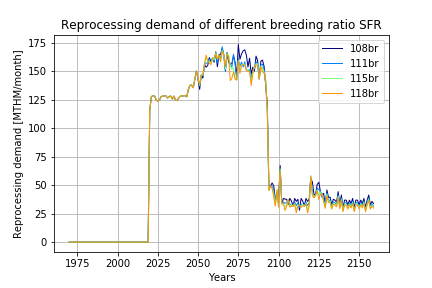
\includegraphics[scale=0.6]{./images/sensitivity/br_tot_rep.png}
    \end{center}
    \caption{Increasing the breeding ratio decreases the monthly reprocessing 
    demand.}
    \label{fig:br_rep}
\end{figure}

The sensitivity analysis also shows, as demonstrated in \cref{fig:br_uox} that 
increasing the breeding ratio decreases the mass of \gls{UOX} \gls{UNF} 
required for the transition. The \glspl{ASTRID} produce more plutonium, reducing the plutonium demand from reprocessed \gls{UOX}. However, since \gls{LWR} \gls{UNF} is not
the limiting factor, increasing the breeding ratio does not play a significant
role in the transition scenario, especially considering the technical difficulty
in achieving a high breeding ratio.

\begin{figure}[htbp!]
    \begin{center}
        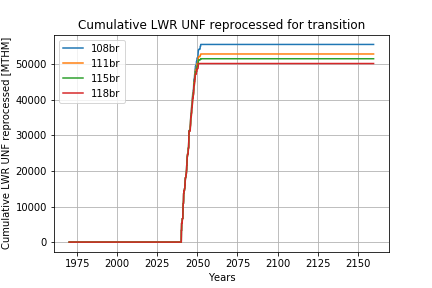
\includegraphics[scale=0.6]{./images/sensitivity/br_uox_unf_cum.png}
    \end{center}
    \caption{Sensitivity analysis demonstrates that increasing the breeding 
    ratio decreases the required \gls{UOX} \gls{UNF}. }
    \label{fig:br_uox}
\end{figure}

The differences between varying breeding ratios are
shown in table \ref{tab:br_diff}. The difference were calculated
using the following equation:

\[ \epsilon = \frac{(x - x_{base})}{x_base} * 100 \]

\begin{table}[h]
	\centering
	\caption{Percent difference of total \gls{LWR} \gls{UNF} reprocessed
		for transition and total reprocessing demand for the simulation.}
	\begin{tabular}{lrrrr}
		\hline
		\multirow{2}{*}{\textbf{Parameter}} & \multicolumn{4}{c}{\% Difference} \\
		 & \textbf{1.08}& \textbf{1.11} & \textbf{1.15} & \textbf{1.18} \\
		\hline
		Total reprocessing demand & 0.0 & -1.8 & -2.6 & -3.4 \\ 
		\gls{LWR} \gls{UNF} reprocessed & 0.0  & -4.9 & -8.0 & -9.7 \\
		\hline
	\end{tabular}
	\label{tab:br_diff}
\end{table}


\subsection{Lifetime Extension of French \glspl{LWR}}\label{sec:life}
Extending the lifetime of French \glspl{LWR} lowers the average
monthly \gls{UOX} reprocessing demand, since the \gls{ASTRID} deployment becomes 
delayed (shown in figure \ref{fig:pow_diff}). The plutonium demand is delayed,
 allowing the reprocessing plant more time to prepare plutonium for \gls{ASTRID} reactors.

\begin{figure}[htbp!]
    \begin{center}
        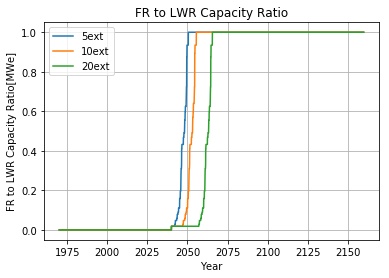
\includegraphics[scale=0.7]{./images/sensitivity/pow_ratio.png}
    \end{center}
    \caption{The ratio of \glspl{ASTRID} to \glspl{LWR} in France demarcates 
    the transition period.}
    \label{fig:pow_diff}
\end{figure}

Figure \ref{fig:ext_uox} shows the decrease in the average monthly
\gls{UOX} reprocessing burden with increased \gls{LWR} lifetimes.
However, the duration of \gls{LWR} \gls{UNF} reprocessing increases,
due to a delay in \gls{SFR} \gls{UNF} generation, which increases
the total amount of \gls{LWR} \gls{UNF} reprocessed (shown in table
\ref{tab:ext_diff}).


\begin{figure}[htbp!]
	\begin{center}
		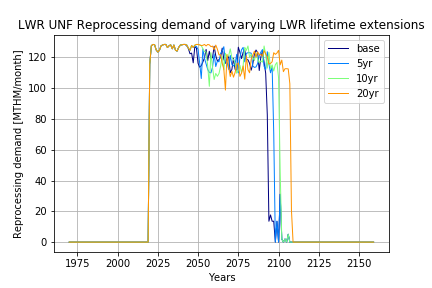
\includegraphics[scale=0.7]{./images/sensitivity/ext_uox_rep.png}
	\end{center}
	\caption{Increasing the lifetime of French \glspl{LWR} decreases the monthly
		\gls{UOX} reprocessing demand, but increases the duration of \gls{LWR} \gls{UNF}
		reprocessing, thereby increasing the total amount of \gls{LWR} \gls{UNF} reprocessed.}
	\label{fig:ext_uox}
\end{figure}

Figure \ref{fig:ext_all} shows that lifetime extension has little
effect on the average total monthly reprocessing demand, because
the amount of plutonium in the \gls{ASTRID} used fuel remains the same.
The delay of \gls{ASTRID} deployment simply provides more time for
France to prepare the fuel. 
The longer lifetimes of \glspl{LWR} delay transition, and gives France
time to accumulate \gls{LWR} \gls{UNF}. However, it does not reduce
the total reprocessing capacity required for transition.



\begin{figure}[htbp!]
    \begin{center}
        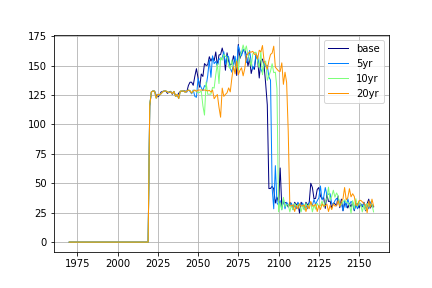
\includegraphics[scale=0.7]{./images/sensitivity/ext_tot_rep.png}
    \end{center}
    \caption{Increasing the lifetime of French \glspl{LWR} simply delays the
             reprocessing demand, and has little impact on the total 
     reprocessing capacity required.}
    \label{fig:ext_all}
\end{figure}

\begin{table}[h]
	\centering
	\caption{Percent difference of total \gls{LWR} \gls{UNF} reprocessed
		for transition and total reprocessing demand for the simulation.}
	\begin{tabular}{lrrrr}
		\hline
		\multirow{2}{*}{\textbf{Parameter}} & \multicolumn{4}{c}{\% Difference} \\
		& \textbf{base}& \textbf{5 years} & \textbf{10 years} & \textbf{20 years} \\
		\hline
		Total reprocessing demand & 0.0 & -5.9 & -3.3 & 3.1 \\
		\gls{LWR} \gls{UNF} reprocessed & 0.0  & 4.2 & 8.6 & 17.8 \\
		\hline
	\end{tabular}
	\label{tab:ext_diff}
\end{table}

